\documentclass{article}
\usepackage[a4paper,left=3cm, right=3cm, top=2cm, bottom=2cm]{geometry}
\usepackage{amsmath}
\usepackage{graphicx}
\usepackage{caption}
\usepackage{setspace}
\usepackage{xcolor}
\usepackage{titlesec}
\usepackage{amssymb}
\graphicspath{{graph/}}
\title{10.1 Curves Defined by Parametric Equations}
\date{}
\author{}
\setstretch{1.2} 

% \subsection* 형식 지정 (번호 없음)
\titleformat{name=\section, numberless}
  {\normalfont\large\bfseries\color{blue}}
  {}
  {0pt}
  {}
\geometry{a4paper, margin=1in}

\begin{document}
\maketitle
\section*{Parametric Equations}
Traditionally, plane curves are described by equations of the form $y=f(x)$, $x=g(y)$, or by an implicit relation $f(x,y)=0$. However, some curves are better described when both $x$ and $y$ are given in terms of a third variable, $t$, called a parameter. These equations are known as parametric equations:
\begin{align*}
    x &= f(t) \\
    y &= g(t)
\end{align*}
Each value of $t$ determines a point $(x,y)$, which can be plotted in a coordinate plane. As $t$ varies, the point $(x,y)=(f(t),g(t))$ traces out a curve called a parametric curve. The parameter $t$ does not necessarily represent time, but in many applications, it does, and $(f(t),g(t))$ can be interpreted as the position of a moving object at time $t$.

The process of finding a Cartesian equation in $x$ and $y$ whose graph coincides with the curve represented by parametric equations is called \textbf{eliminating the parameter}. 
\\While this can be helpful in identifying the shape of the curve, it often results in a loss of information, such as the direction of motion or the particle's position at a given time.
\\If the parameter $t$ is restricted to an interval $a \le t \le b$, the curve has an initial point $(f(a),g(a))$ and a terminal point $(f(b),g(b))$.
\begin{figure}[htbp]
    \centering
    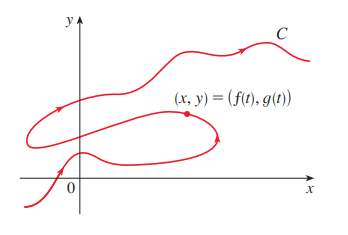
\includegraphics[width=0.3\textwidth]{graph10.png}
    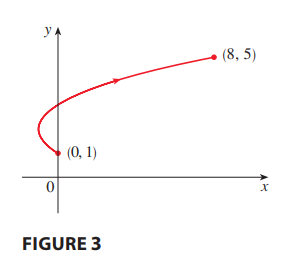
\includegraphics[width=0.3\textwidth]{graph11.png}  % <-- 실제 이미지 파일명으로 변경
\end{figure}

\paragraph{NOTE:} Different parametric equations can represent the same curve. Therefore, a distinction is made between a curve (a set of points) and a parametric curve (where points are traced out in a specific way).

\subsubsection*{EXAMPLE 1}
Sketch and identify the curve defined by the parametric equations $x = t^2 - 2t$, $y = t + 1$.

\paragraph{Solution:} We can create a table of values for $t$, $x$, and $y$:

Plotting these points and connecting them suggests a parabola. To confirm, we eliminate the parameter. From $y=t+1$, we get $t=y-1$. Substituting this into the equation for $x$:
\begin{align*}
    x &= (y-1)^2 - 2(y-1) \\
    x &= (y^2 - 2y + 1) - (2y - 2) \\
    x &= y^2 - 4y + 3
\end{align*}
This is the equation of a parabola. Since $t$ can be any real number, $y$ can also be any real number, so the parametric equations represent the entire parabola. The arrows on the sketched curve indicate the direction of motion as $t$ increases.
\begin{figure}[htbp]
    \centering
    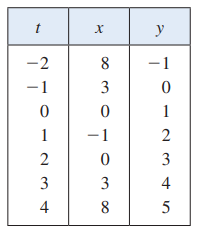
\includegraphics[width=0.2\textwidth]{graph13.png}
    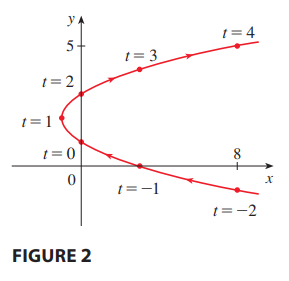
\includegraphics[width=0.3\textwidth]{graph12.png} % <-- 실제 이미지 파일명으로 변경
\end{figure}

\subsubsection*{EXAMPLE 2}
What curve is represented by the following parametric equations? $x=\cos t$, $y=\sin t$, $0 \le t \le 2\pi$.

\paragraph{Solution:} We can eliminate the parameter by using the identity $\cos^2 t + \sin^2 t = 1$.
\[
x^2 + y^2 = (\cos t)^2 + (\sin t)^2 = 1
\]
This is the equation of a unit circle centered at the origin. As $t$ increases from $0$ to $2\pi$, the point $(x,y)=(\cos t, \sin t)$ moves once around the circle in the counterclockwise direction, starting from $(1,0)$.

\subsubsection*{EXAMPLE 3}
What curve is represented by the given parametric equations? $x=\sin 2t$, $y=\cos 2t$, $0 \le t \le 2\pi$.

\paragraph{Solution:} Similar to Example 2, we use the identity $\sin^2\theta + \cos^2\theta = 1$.
\[
x^2 + y^2 = (\sin 2t)^2 + (\cos 2t)^2 = 1
\]
This also represents the unit circle. However, as $t$ increases from $0$ to $2\pi$, the argument $2t$ goes from $0$ to $4\pi$. This means the point $(x,y)=(\sin 2t, \cos 2t)$ starts at $(0,1)$ and moves twice around the circle in the clockwise direction.

\subsubsection*{EXAMPLE 4}
Find parametric equations for the circle with center $(h,k)$ and radius $r$.

\paragraph{Solution:} Starting from the parametric equations for a unit circle centered at the origin ($x=\cos t$, $y=\sin t$), we can scale by $r$ and then shift by $(h,k)$:
\[
x = h + r\cos t \qquad y = k + r\sin t \qquad \text{for } 0 \le t \le 2\pi.
\]
\begin{figure}[htbp]
    \centering
    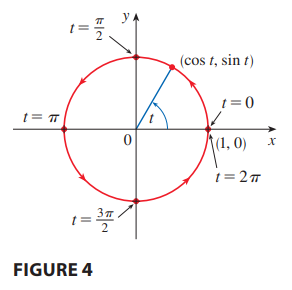
\includegraphics[width=0.3\textwidth]{graph19.png}
    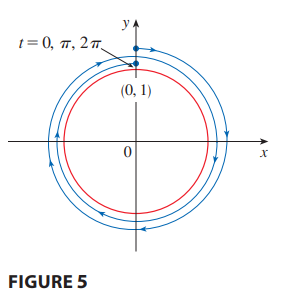
\includegraphics[width=0.3\textwidth]{graph20.png}
    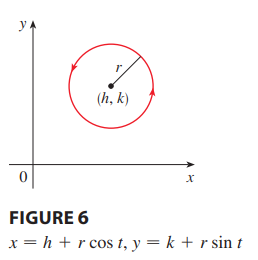
\includegraphics[width=0.3\textwidth]{graph21.png}
\end{figure}

\subsubsection*{EXAMPLE 5}
Each of the following sets of parametric equations gives the position of a moving particle at time $t$.
\begin{enumerate}
    \item[(a)] $x=t^3, y=t$
    \item[(b)] $x=-t^3, y=-t$
    \item[(c)] $x=t^{3/2}, y=\sqrt{t}$
    \item[(d)] $x=e^{-3t}, y=e^{-t}$
\end{enumerate}

\paragraph{Solution:} In each case, eliminating the parameter gives $x=y^3$, so each particle moves along the cubic curve $x=y^3$. However, the particles move in different ways:
\begin{enumerate}
    \item[(a)] The particle moves from left to right as $t$ increases.
    \item[(b)] The particle moves from right to left as $t$ increases.
    \item[(c)] The equations are defined only for $t \ge 0$. The particle starts at the origin and moves to the right.
    \item[(d)] Here $x>0$ and $y>0$. The particle approaches the origin as $t$ increases.
\end{enumerate}

\begin{figure}[htbp]
    \centering
    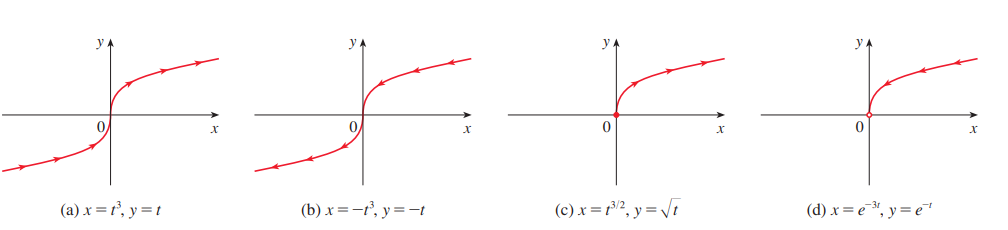
\includegraphics[width=1\textwidth]{graph22.png} % <-- 실제 이미지 파일명으로 변경
\end{figure}

\subsubsection*{EXAMPLE 6}
Sketch the curve with parametric equations $x=\sin t, y=\sin^2 t$.

\paragraph{Solution:} Observe that $y = (\sin t)^2 = x^2$. So the point $(x,y)$ moves on the parabola $y=x^2$. However, since $-1 \le \sin t \le 1$, we have $-1 \le x \le 1$. Therefore, the parametric equations represent only the part of the parabola for which $-1 \le x \le 1$. Since $\sin t$ is periodic, the point $(x,y)=(\sin t, \sin^2 t)$ moves back and forth infinitely often along the parabola from $(-1,1)$ to $(1,1)$.

\subsubsection*{EXAMPLE 7}
The curve represented by the parametric equations $x=\cos t, y=\sin 2t$ is shown in Figure 9. It is an example of a Lissajous figure.

\paragraph{Solution:} We see that as $t$ increases from $0$ to $\pi/2$, $x$ decreases from $1$ to $0$ while $y$ starts at $0$, increases to $1$, and then returns to $0$. Together these descriptions produce the portion of the parametric curve that we see in the first quadrant. If we proceed similarly, we get the complete curve. It is possible to eliminate the parameters, but the resulting equation ($y^2 = 4x^2 - 4x^4$) isn’t very helpful.

\begin{figure}[htbp]
    \centering
    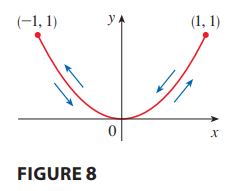
\includegraphics[width=0.2\textwidth]{graph23.png}
    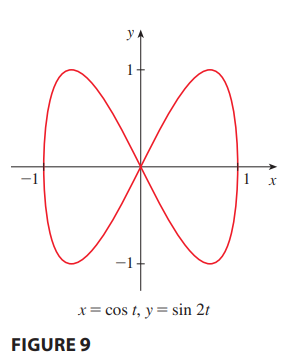
\includegraphics[width=0.23\textwidth]{graph24.png}  % <-- 실제 이미지 파일명으로 변경
\end{figure}

\section*{Graphing Parametric Curves with Technology}
Most graphing software applications and graphing calculators can graph curves defined by parametric equations.

\subsubsection*{EXAMPLE 8}
Use a calculator or computer to graph the curve $x = y^4 - 3y^2$.

\paragraph{Solution:} If we let the parameter be $t=y$, then we have the equations:
\[
x = t^4 - 3t^2 \qquad y=t
\]
Using these parametric equations, we obtain the graph. This method is much easier than solving for $y$ as four functions of $x$ and graphing them individually. In general, to graph an equation of the form $x=g(y)$, we can use the parametric equations $x=g(t), y=t$. Similarly, for $y=f(x)$, we can use $x=t, y=f(t)$.
\begin{figure}[htbp]
    \centering
    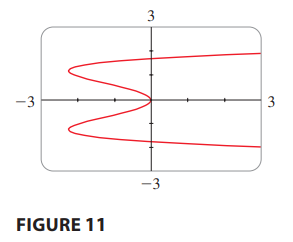
\includegraphics[width=0.25\textwidth]{graph25.png}
    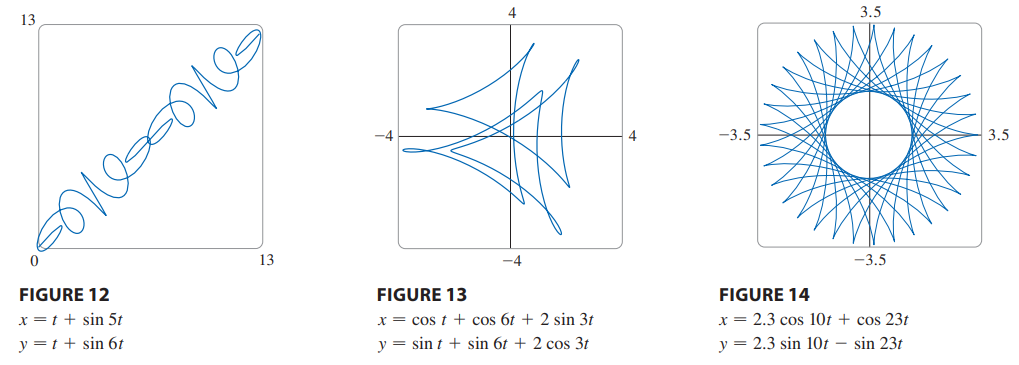
\includegraphics[width=0.6\textwidth]{graph26.png}  % <-- 실제 이미지 파일명으로 변경
\end{figure}

\section*{The Cycloid}
\subsubsection*{EXAMPLE 9}
The curve traced out by a point P on the circumference of a circle as the circle rolls along a straight line is called a cycloid. 
\\If the circle has radius $r$ and rolls along the x-axis and if one position of P is the origin, find parametric equations for the cycloid.

\paragraph{Solution:} We choose the angle of rotation $\theta$ of the circle as the parameter ($\theta=0$ when P is at the origin). The distance the circle has rolled from the origin is $|OT| = \text{arc } PT = r\theta$. The center of the circle is $C(r\theta, r)$. Let the coordinates of P be $(x,y)$. From the geometry:
\begin{align*}
    x &= |OT| - |PQ| = r\theta - r\sin\theta = r(\theta - \sin\theta) \\
    y &= |TC| - |QC| = r - r\cos\theta = r(1 - \cos\theta)
\end{align*}
Therefore, the parametric equations of the cycloid are:
\[
 x = r(\theta - \sin\theta), \qquad y = r(1 - \cos\theta) \qquad \text{for } \theta \in {R}
\]
One arch of the cycloid is described by $0 \le \theta \le 2\pi$.
\begin{figure}[htbp]
    \centering
    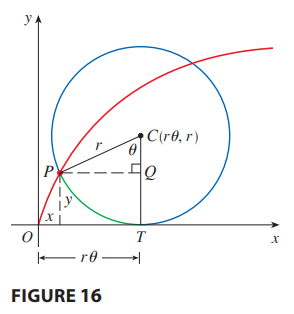
\includegraphics[width=0.3\textwidth]{graph14.png}
    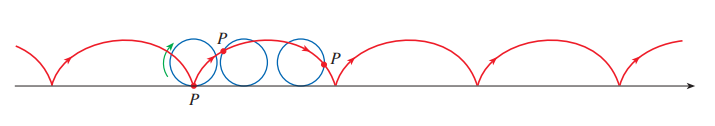
\includegraphics[width=0.6\textwidth]{graph18.png}
\end{figure}

\paragraph{Brachistochrone Problem:} Find the curve along which a particle slides from point A to point B (not directly below A) in the shortest time under gravity. John Bernoulli (1696) solved this and proved that the curve of fastest descent is an inverted arch of a cycloid.

\paragraph{Tautochrone Problem:} Huygens (1673) showed that the cycloid is also the solution to the tautochrone problem, meaning: A particle P on an inverted cycloid will always take the same time to reach the bottom, regardless of starting position.
\begin{figure}[htbp]
    \centering
    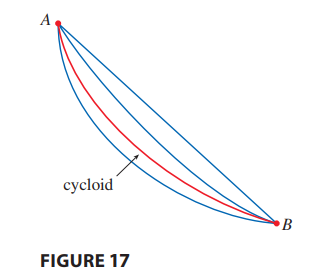
\includegraphics[width=0.25\textwidth]{graph15.png}
    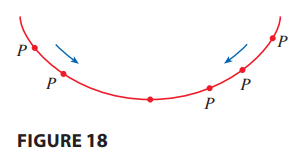
\includegraphics[width=0.25\textwidth]{graph16.png}
\end{figure}


\section*{Families of Parametric Curves}
\subsubsection*{EXAMPLE 10}
Investigate the family of curves with parametric equations $x=a+\cos t, y=a\tan t+\sin t$. What do these curves have in common? How does the shape change as $a$ increases?

\paragraph{Solution:} These curves are called conchoids of Nicomedes. They all have two branches (except for $a=0$) and both branches approach the vertical asymptote $x=a$.
\\When $a < -1$, both branches are smooth.\\ When $a=-1$, the right branch acquires a sharp point (cusp). 
\\For $-1 < a < 0$, the cusp turns into a loop, which becomes larger as $a$ approaches $0$. When $a=0$, both branches come together and form a circle ($x=\cos t, y=\sin t$). 
\\For $0 < a < 1$, the left branch has a loop, which shrinks to become a cusp when $a=1$. 
\\For $a>1$, the branches become smooth again, and as $a$ increases further, they become less curved. The curves with positive $a$ are reflections about the y-axis of the corresponding curves with negative $a$.
\begin{figure}[htbp]
    \centering
    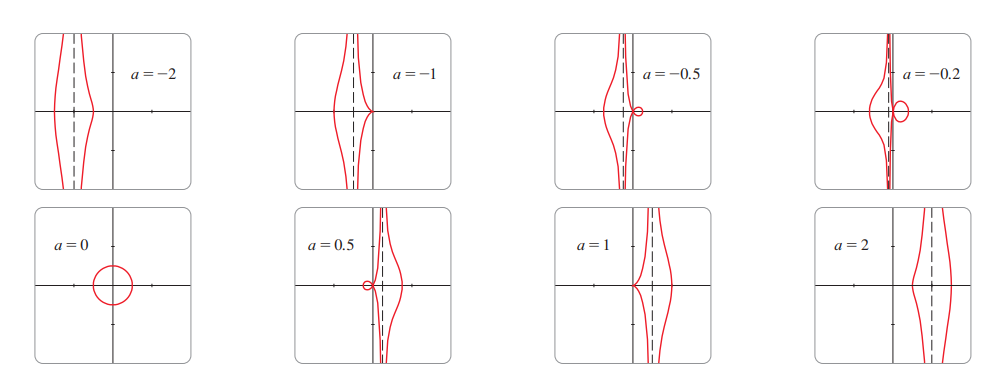
\includegraphics[width=1\textwidth]{graph17.png}
\end{figure}
\end{document}
